\newpage
\section{Resultados}

\subsection{Questão 1}

Seguindo as instruções da questão 1, foi obtido a imagem \ref{fig:q1}. Como pode ser visto na imagem, a frequência de saída é de $f = 103,73 kHz$.

\begin{figure}[H]
    \centering
    \caption{Forma de onda no controlador.}
    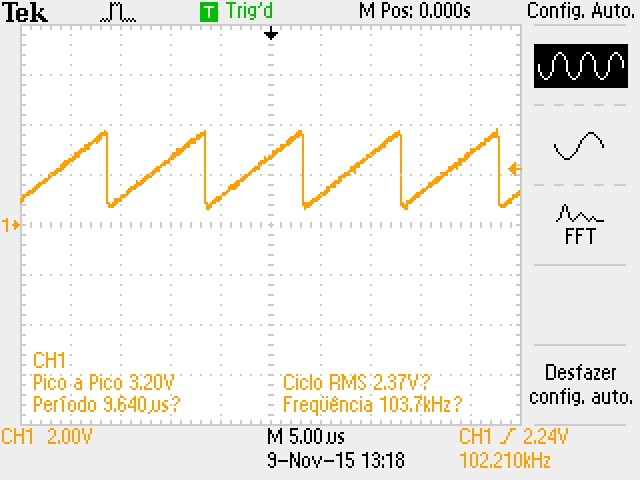
\includegraphics[scale=0.8]{q1}
    \label{fig:q1}
\end{figure}

Para $K_c = 1$, a frequência de saída é dobrada. Sendo assim, $f = 207,46 kHz$.

\subsection{Questão 2}

Como pode ser visto na figura \ref{fig:q2}, a frequência de saída é de 56 kHz.

\begin{figure}[H]
    \centering
    \caption{Forma de onda na saída controlador (aprox. 50 kHz).}
    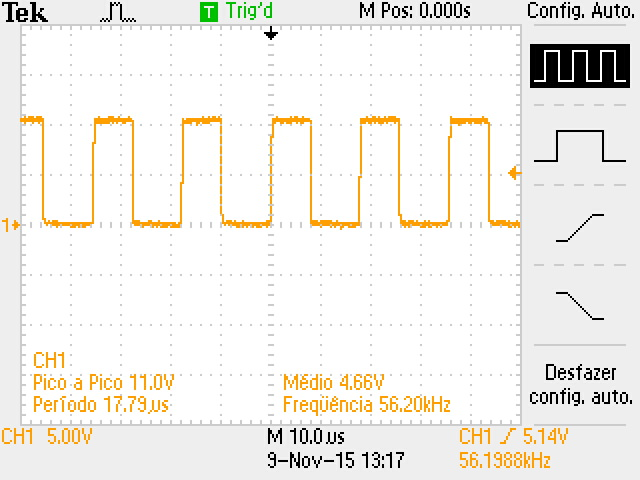
\includegraphics[scale=0.8]{q2}
    \label{fig:q2}
\end{figure}

Fazendo $K_c = 1$, a frequência de saída passa para 108 kHz.

\subsection{Questão 3}
Utilizando o ferro de solda próximo ao termistor, foi possível notar que, quando a temperatura no NTC atinge um determinado valor, o conversor é desligado. Quando a temperatura começa a diminuir, o conversor volta a funcionar, dando um "tranco" no conversor e gerando uma alta corrente inicial.

\subsection{Questão 4}
 A tensão de saída mensurada foi de 13,02 V.
 
\subsection{Questão 5}
A tensão de saída mensurada foi de 25,6V

\subsection{Questão 6}
Os conversores que possuem duas chaves.
\begin{itemize}
    \item \textit{Forward 2T}.
    \item \textit{Push-Pull}.
    \item \textit{Half-Bridge}.
\end{itemize}

\subsection{Questão 7}
Conversores que possuem somente uma chave e aceitam razão cíclica maior que 50\%.

\begin{itemize}
    \item \textit{Buck}.
    \item \textit{Boost}.
    \item \textit{Flyback}.
\end{itemize}